\section[CNNs]{Convolutional neural networks}

\subsection{}

\begin{frame}
    \frametitle{Motivation}

    \begin{block}{Disclaimer}
        I know almost nothing about CNNs, but not discussing them would be sacrilegious.
        I'll do my best.
    \end{block}

    \begin{itemize}
        \item Much of deep learning revolves around image classification
        \item A huge proportion of early major breakthroughs in deep learning involved CNNs for image classification
    \end{itemize}

    \begin{block}{Spatial invariance}
        CNNs leverage the fact that images are \alert{spatially invariant}
        \begin{itemize}
            \item A dog is a dog whether its head is in the left or right side of an image
            \item Dense networks treat every input as independent
        \end{itemize}
    \end{block}
\end{frame}

\begin{frame}
    \frametitle{Rich history that authors expect you to know}
    \begin{columns}
        \begin{column}{0.55\textwidth}
            \begin{itemize}
                \item<+-> Late 1990s: MNIST database of handwritten digits
                \begin{itemize}
                    \item 60,000 training samples, 10,000 test samples
                    \item $28 \times 28$ pixels, black and white
                    \item CNN test error: 0.7\% \citep[``LeNet-5'',][]{LeCunIEEE98} to 0.21\% \citep{WanICML13}
                \end{itemize}
                \item<+-> Early 2010s: CIFAR-10/100 database, 10/100 image labels
                \begin{itemize}
                    \item 50,000 training samples, 10,000 test samples
                    \item $32 \times 32$ color images
                    \item CIFAR-10 test error: 35\% \citep{RanzatoAISTATS10} to 2.1\% \citep{Real18}
                \end{itemize}
                \item Early 2010s: ImageNet---$\O(10^7)$ images, $\O(10^4)$ labels
            \end{itemize}
        \end{column}
        \begin{column}{0.45\textwidth}
            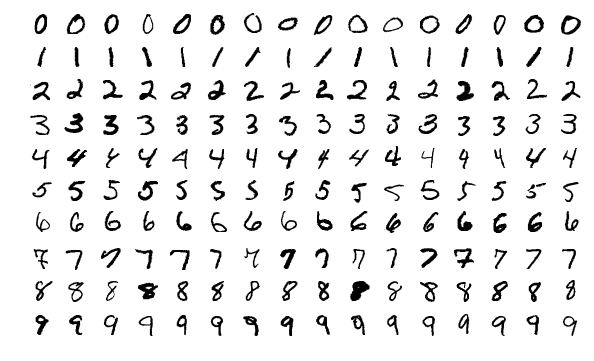
\includegraphics[width=\textwidth]{mnist} \\[5mm]
            \uncover<.->{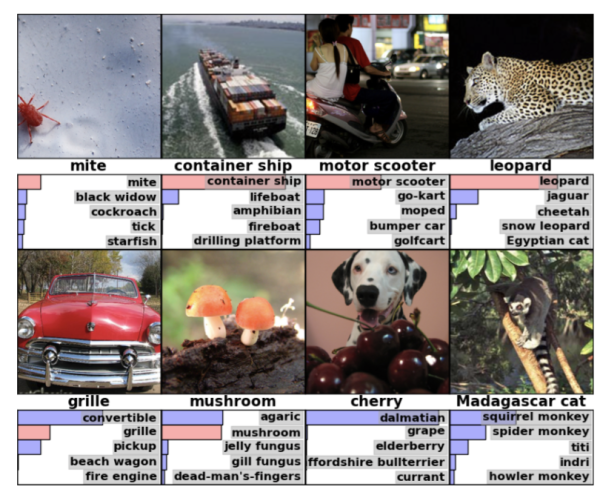
\includegraphics[width=\textwidth]{imagenet}}
        \end{column}
    \end{columns}
\end{frame}

\begin{frame}
    \frametitle{CNN architectures that authors expect you to know}

    \begin{itemize}
        \item LeNet \citep{LeCunIEEE98}
        \item AlexNet \citep{KrizhevskyNIPS12}
        \item VGGNet \citep{Simonyan14}
        \item GoogLeNet/Inception \citep{SzegedyIEEECVPR15}
        \item ResNet \citep{He15b}
    \end{itemize}
\end{frame}

%%% Local Variables:
%%% mode: latex
%%% TeX-master: "../nn"
%%% End:
